% Generated by Sphinx.
\def\sphinxdocclass{report}
\documentclass[letterpaper,10pt,english]{sphinxmanual}
\usepackage[utf8]{inputenc}
\DeclareUnicodeCharacter{00A0}{\nobreakspace}
\usepackage{cmap}
\usepackage[T1]{fontenc}
\usepackage{babel}
\usepackage{times}
\usepackage[Bjarne]{fncychap}
\usepackage{longtable}
\usepackage{sphinx}
\usepackage{multirow}

\addto\captionsenglish{\renewcommand{\figurename}{Fig. }}
\addto\captionsenglish{\renewcommand{\tablename}{Table }}
\floatname{literal-block}{Listing }



\title{pygot Documentation}
\date{April 28, 2015}
\release{0.1.0}
\author{Edwin Tye}
\newcommand{\sphinxlogo}{}
\renewcommand{\releasename}{Release}
\makeindex

\makeatletter
\def\PYG@reset{\let\PYG@it=\relax \let\PYG@bf=\relax%
    \let\PYG@ul=\relax \let\PYG@tc=\relax%
    \let\PYG@bc=\relax \let\PYG@ff=\relax}
\def\PYG@tok#1{\csname PYG@tok@#1\endcsname}
\def\PYG@toks#1+{\ifx\relax#1\empty\else%
    \PYG@tok{#1}\expandafter\PYG@toks\fi}
\def\PYG@do#1{\PYG@bc{\PYG@tc{\PYG@ul{%
    \PYG@it{\PYG@bf{\PYG@ff{#1}}}}}}}
\def\PYG#1#2{\PYG@reset\PYG@toks#1+\relax+\PYG@do{#2}}

\expandafter\def\csname PYG@tok@gd\endcsname{\def\PYG@tc##1{\textcolor[rgb]{0.63,0.00,0.00}{##1}}}
\expandafter\def\csname PYG@tok@gu\endcsname{\let\PYG@bf=\textbf\def\PYG@tc##1{\textcolor[rgb]{0.50,0.00,0.50}{##1}}}
\expandafter\def\csname PYG@tok@gt\endcsname{\def\PYG@tc##1{\textcolor[rgb]{0.00,0.27,0.87}{##1}}}
\expandafter\def\csname PYG@tok@gs\endcsname{\let\PYG@bf=\textbf}
\expandafter\def\csname PYG@tok@gr\endcsname{\def\PYG@tc##1{\textcolor[rgb]{1.00,0.00,0.00}{##1}}}
\expandafter\def\csname PYG@tok@cm\endcsname{\let\PYG@it=\textit\def\PYG@tc##1{\textcolor[rgb]{0.25,0.50,0.56}{##1}}}
\expandafter\def\csname PYG@tok@vg\endcsname{\def\PYG@tc##1{\textcolor[rgb]{0.73,0.38,0.84}{##1}}}
\expandafter\def\csname PYG@tok@m\endcsname{\def\PYG@tc##1{\textcolor[rgb]{0.13,0.50,0.31}{##1}}}
\expandafter\def\csname PYG@tok@mh\endcsname{\def\PYG@tc##1{\textcolor[rgb]{0.13,0.50,0.31}{##1}}}
\expandafter\def\csname PYG@tok@cs\endcsname{\def\PYG@tc##1{\textcolor[rgb]{0.25,0.50,0.56}{##1}}\def\PYG@bc##1{\setlength{\fboxsep}{0pt}\colorbox[rgb]{1.00,0.94,0.94}{\strut ##1}}}
\expandafter\def\csname PYG@tok@ge\endcsname{\let\PYG@it=\textit}
\expandafter\def\csname PYG@tok@vc\endcsname{\def\PYG@tc##1{\textcolor[rgb]{0.73,0.38,0.84}{##1}}}
\expandafter\def\csname PYG@tok@il\endcsname{\def\PYG@tc##1{\textcolor[rgb]{0.13,0.50,0.31}{##1}}}
\expandafter\def\csname PYG@tok@go\endcsname{\def\PYG@tc##1{\textcolor[rgb]{0.20,0.20,0.20}{##1}}}
\expandafter\def\csname PYG@tok@cp\endcsname{\def\PYG@tc##1{\textcolor[rgb]{0.00,0.44,0.13}{##1}}}
\expandafter\def\csname PYG@tok@gi\endcsname{\def\PYG@tc##1{\textcolor[rgb]{0.00,0.63,0.00}{##1}}}
\expandafter\def\csname PYG@tok@gh\endcsname{\let\PYG@bf=\textbf\def\PYG@tc##1{\textcolor[rgb]{0.00,0.00,0.50}{##1}}}
\expandafter\def\csname PYG@tok@ni\endcsname{\let\PYG@bf=\textbf\def\PYG@tc##1{\textcolor[rgb]{0.84,0.33,0.22}{##1}}}
\expandafter\def\csname PYG@tok@nl\endcsname{\let\PYG@bf=\textbf\def\PYG@tc##1{\textcolor[rgb]{0.00,0.13,0.44}{##1}}}
\expandafter\def\csname PYG@tok@nn\endcsname{\let\PYG@bf=\textbf\def\PYG@tc##1{\textcolor[rgb]{0.05,0.52,0.71}{##1}}}
\expandafter\def\csname PYG@tok@no\endcsname{\def\PYG@tc##1{\textcolor[rgb]{0.38,0.68,0.84}{##1}}}
\expandafter\def\csname PYG@tok@na\endcsname{\def\PYG@tc##1{\textcolor[rgb]{0.25,0.44,0.63}{##1}}}
\expandafter\def\csname PYG@tok@nb\endcsname{\def\PYG@tc##1{\textcolor[rgb]{0.00,0.44,0.13}{##1}}}
\expandafter\def\csname PYG@tok@nc\endcsname{\let\PYG@bf=\textbf\def\PYG@tc##1{\textcolor[rgb]{0.05,0.52,0.71}{##1}}}
\expandafter\def\csname PYG@tok@nd\endcsname{\let\PYG@bf=\textbf\def\PYG@tc##1{\textcolor[rgb]{0.33,0.33,0.33}{##1}}}
\expandafter\def\csname PYG@tok@ne\endcsname{\def\PYG@tc##1{\textcolor[rgb]{0.00,0.44,0.13}{##1}}}
\expandafter\def\csname PYG@tok@nf\endcsname{\def\PYG@tc##1{\textcolor[rgb]{0.02,0.16,0.49}{##1}}}
\expandafter\def\csname PYG@tok@si\endcsname{\let\PYG@it=\textit\def\PYG@tc##1{\textcolor[rgb]{0.44,0.63,0.82}{##1}}}
\expandafter\def\csname PYG@tok@s2\endcsname{\def\PYG@tc##1{\textcolor[rgb]{0.25,0.44,0.63}{##1}}}
\expandafter\def\csname PYG@tok@vi\endcsname{\def\PYG@tc##1{\textcolor[rgb]{0.73,0.38,0.84}{##1}}}
\expandafter\def\csname PYG@tok@nt\endcsname{\let\PYG@bf=\textbf\def\PYG@tc##1{\textcolor[rgb]{0.02,0.16,0.45}{##1}}}
\expandafter\def\csname PYG@tok@nv\endcsname{\def\PYG@tc##1{\textcolor[rgb]{0.73,0.38,0.84}{##1}}}
\expandafter\def\csname PYG@tok@s1\endcsname{\def\PYG@tc##1{\textcolor[rgb]{0.25,0.44,0.63}{##1}}}
\expandafter\def\csname PYG@tok@gp\endcsname{\let\PYG@bf=\textbf\def\PYG@tc##1{\textcolor[rgb]{0.78,0.36,0.04}{##1}}}
\expandafter\def\csname PYG@tok@sh\endcsname{\def\PYG@tc##1{\textcolor[rgb]{0.25,0.44,0.63}{##1}}}
\expandafter\def\csname PYG@tok@ow\endcsname{\let\PYG@bf=\textbf\def\PYG@tc##1{\textcolor[rgb]{0.00,0.44,0.13}{##1}}}
\expandafter\def\csname PYG@tok@sx\endcsname{\def\PYG@tc##1{\textcolor[rgb]{0.78,0.36,0.04}{##1}}}
\expandafter\def\csname PYG@tok@bp\endcsname{\def\PYG@tc##1{\textcolor[rgb]{0.00,0.44,0.13}{##1}}}
\expandafter\def\csname PYG@tok@c1\endcsname{\let\PYG@it=\textit\def\PYG@tc##1{\textcolor[rgb]{0.25,0.50,0.56}{##1}}}
\expandafter\def\csname PYG@tok@kc\endcsname{\let\PYG@bf=\textbf\def\PYG@tc##1{\textcolor[rgb]{0.00,0.44,0.13}{##1}}}
\expandafter\def\csname PYG@tok@c\endcsname{\let\PYG@it=\textit\def\PYG@tc##1{\textcolor[rgb]{0.25,0.50,0.56}{##1}}}
\expandafter\def\csname PYG@tok@mf\endcsname{\def\PYG@tc##1{\textcolor[rgb]{0.13,0.50,0.31}{##1}}}
\expandafter\def\csname PYG@tok@err\endcsname{\def\PYG@bc##1{\setlength{\fboxsep}{0pt}\fcolorbox[rgb]{1.00,0.00,0.00}{1,1,1}{\strut ##1}}}
\expandafter\def\csname PYG@tok@mb\endcsname{\def\PYG@tc##1{\textcolor[rgb]{0.13,0.50,0.31}{##1}}}
\expandafter\def\csname PYG@tok@ss\endcsname{\def\PYG@tc##1{\textcolor[rgb]{0.32,0.47,0.09}{##1}}}
\expandafter\def\csname PYG@tok@sr\endcsname{\def\PYG@tc##1{\textcolor[rgb]{0.14,0.33,0.53}{##1}}}
\expandafter\def\csname PYG@tok@mo\endcsname{\def\PYG@tc##1{\textcolor[rgb]{0.13,0.50,0.31}{##1}}}
\expandafter\def\csname PYG@tok@kd\endcsname{\let\PYG@bf=\textbf\def\PYG@tc##1{\textcolor[rgb]{0.00,0.44,0.13}{##1}}}
\expandafter\def\csname PYG@tok@mi\endcsname{\def\PYG@tc##1{\textcolor[rgb]{0.13,0.50,0.31}{##1}}}
\expandafter\def\csname PYG@tok@kn\endcsname{\let\PYG@bf=\textbf\def\PYG@tc##1{\textcolor[rgb]{0.00,0.44,0.13}{##1}}}
\expandafter\def\csname PYG@tok@o\endcsname{\def\PYG@tc##1{\textcolor[rgb]{0.40,0.40,0.40}{##1}}}
\expandafter\def\csname PYG@tok@kr\endcsname{\let\PYG@bf=\textbf\def\PYG@tc##1{\textcolor[rgb]{0.00,0.44,0.13}{##1}}}
\expandafter\def\csname PYG@tok@s\endcsname{\def\PYG@tc##1{\textcolor[rgb]{0.25,0.44,0.63}{##1}}}
\expandafter\def\csname PYG@tok@kp\endcsname{\def\PYG@tc##1{\textcolor[rgb]{0.00,0.44,0.13}{##1}}}
\expandafter\def\csname PYG@tok@w\endcsname{\def\PYG@tc##1{\textcolor[rgb]{0.73,0.73,0.73}{##1}}}
\expandafter\def\csname PYG@tok@kt\endcsname{\def\PYG@tc##1{\textcolor[rgb]{0.56,0.13,0.00}{##1}}}
\expandafter\def\csname PYG@tok@sc\endcsname{\def\PYG@tc##1{\textcolor[rgb]{0.25,0.44,0.63}{##1}}}
\expandafter\def\csname PYG@tok@sb\endcsname{\def\PYG@tc##1{\textcolor[rgb]{0.25,0.44,0.63}{##1}}}
\expandafter\def\csname PYG@tok@k\endcsname{\let\PYG@bf=\textbf\def\PYG@tc##1{\textcolor[rgb]{0.00,0.44,0.13}{##1}}}
\expandafter\def\csname PYG@tok@se\endcsname{\let\PYG@bf=\textbf\def\PYG@tc##1{\textcolor[rgb]{0.25,0.44,0.63}{##1}}}
\expandafter\def\csname PYG@tok@sd\endcsname{\let\PYG@it=\textit\def\PYG@tc##1{\textcolor[rgb]{0.25,0.44,0.63}{##1}}}

\def\PYGZbs{\char`\\}
\def\PYGZus{\char`\_}
\def\PYGZob{\char`\{}
\def\PYGZcb{\char`\}}
\def\PYGZca{\char`\^}
\def\PYGZam{\char`\&}
\def\PYGZlt{\char`\<}
\def\PYGZgt{\char`\>}
\def\PYGZsh{\char`\#}
\def\PYGZpc{\char`\%}
\def\PYGZdl{\char`\$}
\def\PYGZhy{\char`\-}
\def\PYGZsq{\char`\'}
\def\PYGZdq{\char`\"}
\def\PYGZti{\char`\~}
% for compatibility with earlier versions
\def\PYGZat{@}
\def\PYGZlb{[}
\def\PYGZrb{]}
\makeatother

\renewcommand\PYGZsq{\textquotesingle}

\begin{document}

\maketitle
\tableofcontents
\phantomsection\label{index::doc}


Contents:


\chapter{Getting started}
\label{getting_started:getting-started}\label{getting_started::doc}\label{getting_started:welcome-to-pygot-s-documentation}\label{getting_started:id1}

\section{What this package do}
\label{getting_started:what-this-package-do}\label{getting_started:package-purpose}
The purpose of this package is to allow the end user to easily define a set of ordinary differential equations (ode) and obtain information about the ode by simply invoking the the appropriate methods.  Here, we define the set of ode's as
\begin{gather}
\begin{split}\frac{\partial \mathbf{x}}{\partial t} = f(\mathbf{x},\boldsymbol{\theta})\end{split}\notag
\end{gather}
where \(\mathbf{x} = \left(x_{1},x_{2},\ldots,x_{n}\right)\) is the state vector with \(d\) state and \(\boldsymbol{\theta}\) the parameters of \(p\) dimension.  Currently, this package allows the end user to find the algebraic expression of the ode, Jacobian, gradient and forward sensitivity of the ode.  A numerical output is given when all the state and parameter values are provided.   Note that the only important class is \code{OperateOdeModel} all the functionality described previously are exposed.

The current plan is to extend the functionality to include
\begin{itemize}
\item {} 
Solving the ode analytically when it is linear

\item {} 
Analysis of the system via eigenvalues during the integration

\item {} 
Detection of DAE

\end{itemize}


\section{Obtaining the package}
\label{getting_started:obtaining-the-package}\label{getting_started:installing-docdir}
The package is currently organized as follows:

\begin{Verbatim}[commandchars=\\\{\}]
pygenericodemodel/
    bin/
    doc/
    pygot/
        direct/
            tests/
        gradient/
            tests/
        optutils/
    LICENSE.txt
    MANIFEST.in
    setup.py
    README.rst
\end{Verbatim}

with files in each of the three main folder not shown.  You can install the package via command line:

\begin{Verbatim}[commandchars=\\\{\}]
python setup.py install
\end{Verbatim}

or locally on a user level:

\begin{Verbatim}[commandchars=\\\{\}]
python setup.py install \PYGZhy{}\PYGZhy{}user
\end{Verbatim}

Unfortunately, the package is not currently uploaded to the Python ecosystem so it cannot be installed via \code{pip} or \code{easy\_install}.  Once the package has gone past the stage of heavy development, it will be made more accessible.

Please note that there are current redundant file are kept under \code{bin/workingScript} for development purpose for the time being.


\section{Testing the package}
\label{getting_started:id2}\label{getting_started:testing-the-package}
Testing can be performed prior or after the installation.  Some standard test files can be found in their respective folder and they can be run in the command line:

\begin{Verbatim}[commandchars=\\\{\}]
python setup.py test
\end{Verbatim}

which can be performed prior to installing the package if desired.


\chapter{DIRECT}
\label{direct::doc}\label{direct:direct}\label{direct:id1}
DIviding RECTangle is a well known method in global optimization.  We have implemented here with a few tweaks and ideas of our own


\section{Setup}
\label{direct:setup}
First, we are going to load the required modules and also define our objective function - the Rosenbrock function.  We use a set of relatively conservative bounds \(x \in [-2,2]^{2}\)

\begin{Verbatim}[commandchars=\\\{\}]
\PYG{g+gp}{In [1]: }\PYG{k+kn}{from} \PYG{n+nn}{pygot.direct} \PYG{k+kn}{import} \PYG{n}{directAlg}\PYG{p}{,} \PYG{n}{optimTestFun}\PYG{p}{,} \PYG{n}{plotDirectBox}\PYG{p}{,} \PYG{n}{IdConditionType}

\PYG{g+gp}{In [2]: }\PYG{k+kn}{import} \PYG{n+nn}{numpy}

\PYG{g+gp}{In [3]: }\PYG{n}{boundSize} \PYG{o}{=} \PYG{l+m+mi}{2}

\PYG{g+gp}{In [4]: }\PYG{n}{lb} \PYG{o}{=} \PYG{o}{\PYGZhy{}}\PYG{n}{numpy}\PYG{o}{.}\PYG{n}{ones}\PYG{p}{(}\PYG{l+m+mi}{2}\PYG{p}{)} \PYG{o}{*} \PYG{n}{boundSize}

\PYG{g+gp}{In [5]: }\PYG{n}{ub} \PYG{o}{=} \PYG{n}{numpy}\PYG{o}{.}\PYG{n}{ones}\PYG{p}{(}\PYG{l+m+mi}{2}\PYG{p}{)} \PYG{o}{*} \PYG{n}{boundSize}

\PYG{g+gp}{In [6]: }\PYG{n}{func} \PYG{o}{=} \PYG{n}{optimTestFun}\PYG{o}{.}\PYG{n}{rosen}
\end{Verbatim}


\section{Original form}
\label{direct:original-form}
In the seminal paper by Jones et al. it uses an \(\varepsilon\) condition to determine the dividing boxes.  We have to explicitly tell it to use the this condition via \code{IdConditionType()}, which is Soft in this case

\begin{Verbatim}[commandchars=\\\{\}]
\PYG{g+gp}{In [7]: }\PYG{n}{rectListOptim}\PYG{p}{,}\PYG{n}{output} \PYG{o}{=} \PYG{n}{directAlg}\PYG{o}{.}\PYG{n}{directOptim}\PYG{p}{(}\PYG{n}{func}\PYG{p}{,}\PYG{n}{lb}\PYG{p}{,}\PYG{n}{ub}\PYG{p}{,}

\PYG{g+gp}{In [7]: }\PYG{n}{plotDirectBox}\PYG{p}{(}\PYG{n}{rectListOptim}\PYG{p}{,}\PYG{n}{lb}\PYG{p}{,}\PYG{n}{ub}\PYG{p}{,}\PYG{n}{scaleOutput}\PYG{o}{=}\PYG{n+nb+bp}{False}\PYG{p}{)}
\end{Verbatim}

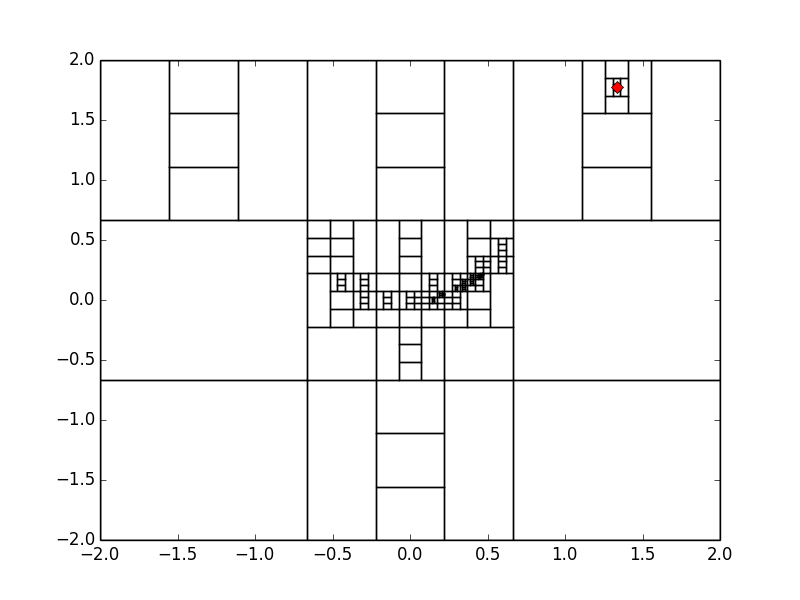
\includegraphics{_static/directSoft.png}

The plots show how the distribution of boxes.  When the condition is not set, by default, it progresses using the Pareto front condition as seen below

\begin{Verbatim}[commandchars=\\\{\}]
\PYG{g+gp}{In [7]: }\PYG{k+kn}{from} \PYG{n+nn}{pygot.direct} \PYG{k+kn}{import} \PYG{n}{directUtil}

\PYG{g+gp}{In [7]: }\PYG{n}{rectListOptim}\PYG{p}{,}\PYG{n}{output} \PYG{o}{=} \PYG{n}{directAlg}\PYG{o}{.}\PYG{n}{directOptim}\PYG{p}{(}\PYG{n}{func}\PYG{p}{,}\PYG{n}{lb}\PYG{p}{,}\PYG{n}{ub}\PYG{p}{,}

\PYG{g+gp}{In [7]: }\PYG{n}{potentialIndex} \PYG{o}{=} \PYG{n}{directUtil}\PYG{o}{.}\PYG{n}{identifyPotentialOptimalObjectPareto}\PYG{p}{(}\PYG{n}{rectListOptim}\PYG{p}{)}

\PYG{g+gp}{In [7]: }\PYG{n}{directUtil}\PYG{o}{.}\PYG{n}{plotParetoFrontRect}\PYG{p}{(}\PYG{n}{rectListOptim}\PYG{p}{,}\PYG{n}{potentialIndex}\PYG{p}{)}
\end{Verbatim}

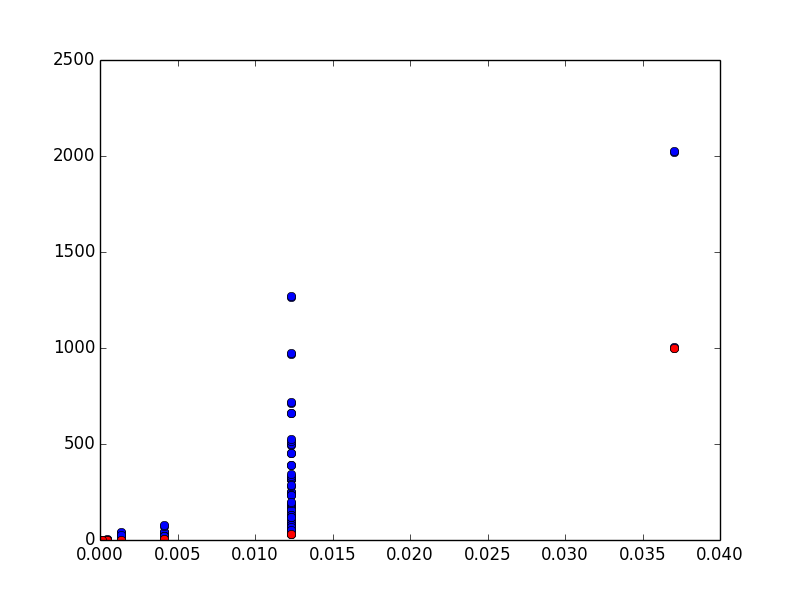
\includegraphics{_static/directParetoFront.png}

In this particular case, the Pareto front condition performs better.  This though, is not a guarantee and using the Pareot front usually result in a lot more function evaluations

\begin{Verbatim}[commandchars=\\\{\}]
\PYG{g+gp}{In [7]: }\PYG{n}{plotDirectBox}\PYG{p}{(}\PYG{n}{rectListOptim}\PYG{p}{,}\PYG{n}{lb}\PYG{p}{,}\PYG{n}{ub}\PYG{p}{,}\PYG{n}{scaleOutput}\PYG{o}{=}\PYG{n+nb+bp}{False}\PYG{p}{)}
\end{Verbatim}

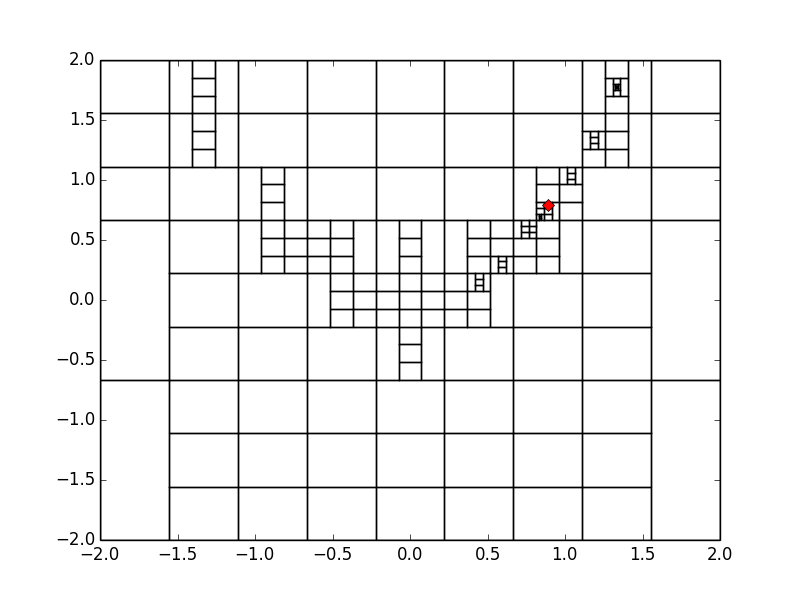
\includegraphics{_static/directPareto.png}


\chapter{Code documentations}
\label{modules/mod:code-documentations}\label{modules/mod::doc}\label{modules/mod:mod}

\section{direct}
\label{modules/mod:direct}

\subsection{direct}
\label{modules/direct::doc}\label{modules/direct:direct}

\begin{fulllineitems}
\pysiglinewithargsret{\strong{class }\code{pygot.direct.directAlg.}\bfcode{direct}}{\emph{func}, \emph{lb}, \emph{ub}, \emph{A=None}, \emph{b=None}, \emph{conditionType=None}, \emph{targetMin=0.0}, \emph{EPSILON=0.0001}, \emph{TOLERENCE=0.0001}}{}~\begin{quote}

DIRECT object
\end{quote}
\begin{quote}\begin{description}
\item[{Parameters}] \leavevmode
\textbf{func: callable}
\begin{quote}
\begin{quote}

objective function
\end{quote}
\begin{description}
\item[{lb: array like}] \leavevmode
lower bounds for the parameters

\item[{ub: array like}] \leavevmode
upper bounds for the parameters

\item[{A: array like, optional}] \leavevmode
matrix of A in Ax\textless{}=b

\item[{b: array like, optional}] \leavevmode
vector of b in Ax\textless{}=b

\item[{conditionType: enum, optional}] \leavevmode
of class \code{IdConditionType}.  Defaults to Pareto like condition
to select the next set of boxes

\item[{targetMin: float, optional}] \leavevmode
the target (best possible) minimum, i.e. 0 for a square/absolute loss

\item[{EPSILON: float, optional}] \leavevmode
parameter to determine how local the search it

\item[{TOLERENCE: float, optional}] \leavevmode
tolerence for

\end{description}
\end{quote}

\textbf{arepsilon-optimal condition}

\end{description}\end{quote}


\begin{fulllineitems}
\pysiglinewithargsret{\bfcode{divide}}{\emph{iteration=50}, \emph{numBox=1000}, \emph{scaleOutput=False}, \emph{full\_output=False}}{}
Dividing up the parameter space with respect to the type of bounds
\begin{quote}\begin{description}
\item[{Parameters}] \leavevmode
\textbf{iteration: int, optional}
\begin{quote}

maximum number of iterations allowed. Defaults to 50
\end{quote}

\textbf{numBox: int, optional}
\begin{quote}

maximum number of boxes allowed. Defaults to 1000
\end{quote}

\textbf{scaleOutput: bool, optional}
\begin{quote}

the rectangles will be scaled to between bounds 0 and 1 if True.  
Note that we scale only when box constraints are present
\end{quote}

\textbf{full\_output: bool, optional}
\begin{quote}

if extra information is required
\end{quote}

\item[{Returns}] \leavevmode
objList: list
\begin{quote}

list of the objects after dividing
\end{quote}

\textbf{infodict} : dict, only returned if full\_output == True
\begin{quote}

Dictionary containing additional output information

\begin{tabulary}{\linewidth}{|L|L|}
\hline
\textsf{\relax 
key
} & \textsf{\relax 
meaning
}\\
\hline
`message'
 & 
reason for stopping
\\
\hline
`fx'
 & 
progress of the objective value
\\
\hline
`iter'
 & 
number of iterations taken
\\
\hline
`scale'
 & 
if the bounds on the output has been scaled
\\
\hline
`newBox'
 & 
number of new box in each iteration
\\
\hline
`numBox'
 & 
final number of box
\\
\hline
`bi'
 & 
index of the box with the smallest objective value
\\
\hline
`x'
 & 
the set of parameters with the smallest objective value
\\
\hline
`mt'
 & 
Different type of moves.
0 = Pareto.
1 = 0 + current object with lowest objective value.
2 = 0 + obj with center in the same direct as the gradient
from previous object with lowest objective value.
3 = 1 + 2
\\
\hline\end{tabulary}

\end{quote}

\end{description}\end{quote}

\end{fulllineitems}



\begin{fulllineitems}
\pysiglinewithargsret{\bfcode{initialDivide}}{}{}
The first divide from the origin
\begin{quote}\begin{description}
\item[{Returns}] \leavevmode
list:
\begin{quote}

a list of objects, either of type \code{PolygonObj} or 
\code{RectangleObj} depending on what type of equalities
were used
\end{quote}

\end{description}\end{quote}

\end{fulllineitems}



\begin{fulllineitems}
\pysiglinewithargsret{\bfcode{initialDividePoly}}{}{}
The first divide from the origin under linear equalities.  This performs
a triangulation on the polygon.
\begin{quote}\begin{description}
\item[{Returns}] \leavevmode
list:
\begin{quote}

a list of objects, of type \code{PolygonObj}
\end{quote}

\end{description}\end{quote}

\end{fulllineitems}



\begin{fulllineitems}
\pysiglinewithargsret{\bfcode{initialDivideRect}}{}{}
The first divide from the origin for box constraints
\begin{quote}\begin{description}
\item[{Returns}] \leavevmode
list:
\begin{quote}

a list of objects, of type \code{RectangleObj}
\end{quote}

\end{description}\end{quote}

\end{fulllineitems}


\end{fulllineitems}



\begin{fulllineitems}
\pysiglinewithargsret{\code{pygot.direct.directAlg.}\bfcode{directOptim}}{\emph{func}, \emph{lb}, \emph{ub}, \emph{iteration=50}, \emph{numBox=200}, \emph{conditionType=None}, \emph{targetMin=0.0}, \emph{EPSILON=0.0001}, \emph{TOLERENCE=0.0001}, \emph{scaleOutput=False}, \emph{full\_output=False}}{}~\begin{quote}

DIRECT algorithm.
\end{quote}
\begin{quote}\begin{description}
\item[{Parameters}] \leavevmode
\textbf{func: callable}
\begin{quote}
\begin{quote}

Cost function
\end{quote}
\begin{description}
\item[{lb: array like}] \leavevmode
lower bounds of the parameters space

\item[{ub: callable}] \leavevmode
upper bounds of the parameters space

\item[{iteration: int}] \leavevmode
maximum number of iterations allowed

\item[{numBox: int}] \leavevmode
maximum number of boxes allowed

\item[{strongCondition: bool}] \leavevmode
if the box selection criteria should be strong

\item[{targetMin: float}] \leavevmode
the target (best possible) minimum, i.e. 0 for
a square/absolute loss

\item[{EPSILON: float}] \leavevmode
parameter to determine how local the search it

\item[{TOLERENCE: float}] \leavevmode
tolerence for :math:{\color{red}\bfseries{}{}`}

\end{description}
\end{quote}

\textbf{arepsilon{}`-optimal condition}
\begin{quote}
\begin{description}
\item[{scaleOutput: bool}] \leavevmode
the rectangles will be scaled to between bounds
0 and 1 if True

\item[{full\_output: bool}] \leavevmode
if extra information is required

\end{description}
\end{quote}

\item[{Returns}] \leavevmode
rectList: list
\begin{quote}
\begin{quote}

list of the rectangles after divide
\end{quote}
\begin{description}
\item[{infodict}] \leavevmode{[}dict, only returned if full\_output == True{]}
Dictionary containing additional output information

\begin{tabulary}{\linewidth}{|L|L|}
\hline
\textsf{\relax 
key
} & \textsf{\relax 
meaning
}\\
\hline
`message'
 & 
reason for stopping
\\
\hline
`iter'
 & 
number of iterations taken
\\
\hline
`scale'
 & 
if the bounds on the output has been scaled
\\
\hline
`numBox'
 & 
final number of box
\\
\hline
`mbi'
 & 
index of the box with the smallest objective
value
\\
\hline\end{tabulary}


\end{description}
\end{quote}

\end{description}\end{quote}

\end{fulllineitems}



\begin{fulllineitems}
\pysigline{\strong{class }\code{pygot.direct.directUtil.}\bfcode{IdConditionType}}
This is an Enum describing the different conditions allowed when identifying
the rectangles with potential.

The following four types of transitions are available.

Pareto = boxes that define the Pareto front of f(x) and size of box

Strong = Strong condition using the estimated Lipschitz constant

Soft = Soft condition using the estimated Lipschitz constant

\end{fulllineitems}



\begin{fulllineitems}
\pysiglinewithargsret{\code{pygot.direct.directUtil.}\bfcode{plotDirectBox}}{\emph{rectList}, \emph{lb}, \emph{ub}, \emph{scaleOutput=False}, \emph{paretoIndex=None}}{}
Plot the boxes return by the DIRECT algorithm given a two dimensional problem.
\begin{quote}\begin{description}
\item[{Parameters}] \leavevmode
\textbf{rectList: list}
\begin{quote}

list of rectangles
\end{quote}

\textbf{lb: array like}
\begin{quote}

lower bounds
\end{quote}

\textbf{ub: array like}
\begin{quote}

upper bounds
\end{quote}

\textbf{scaleOutput: bool}
\begin{quote}

True if the input boxes have been scaled to 0,1
\end{quote}

\end{description}\end{quote}

\end{fulllineitems}



\begin{fulllineitems}
\pysiglinewithargsret{\code{pygot.direct.directUtil.}\bfcode{plotDirectPolygon}}{\emph{polyList}, \emph{paretoIndex=None}, \emph{lb=None}, \emph{ub=None}}{}
Plot the boxes return by the DIRECT algorithm given a two dimensional problem.
\begin{quote}\begin{description}
\item[{Parameters}] \leavevmode
\textbf{polyList: list}
\begin{quote}

list of polygon
\end{quote}

\end{description}\end{quote}

\end{fulllineitems}



\begin{fulllineitems}
\pysiglinewithargsret{\code{pygot.direct.directUtil.}\bfcode{plotParetoFrontRect}}{\emph{rectList}, \emph{paretoIndex=None}}{}
Plot the Pareto front formed by the input boxes
\begin{quote}\begin{description}
\item[{Parameters}] \leavevmode
\textbf{rectList: list}
\begin{quote}

list of rectangles
\end{quote}

\end{description}\end{quote}

\end{fulllineitems}



\begin{fulllineitems}
\pysiglinewithargsret{\code{pygot.direct.directUtil.}\bfcode{plotParetoFrontPoly}}{\emph{polyList}, \emph{paretoIndex=None}}{}
Plot the Pareto front formed by the input boxes
\begin{quote}\begin{description}
\item[{Parameters}] \leavevmode
\textbf{rectList: list}
\begin{quote}

list of rectangles
\end{quote}

\end{description}\end{quote}

\end{fulllineitems}



\begin{fulllineitems}
\pysiglinewithargsret{\strong{class }\code{pygot.direct.polyOperation.}\bfcode{PolygonObj}}{\emph{func}, \emph{A}, \emph{b}, \emph{hullorV=None}}{}
Polygon object
\begin{quote}\begin{description}
\item[{Parameters}] \leavevmode
\textbf{func: callable}
\begin{quote}

objective function
\end{quote}

\textbf{A: array like, optional}
\begin{quote}

matrix of A in Ax\textless{}=b
\end{quote}

\textbf{b: array like, optional}
\begin{quote}

vector of b in Ax\textless{}=b
\end{quote}

\textbf{hullorV: :class:{}`scipy.spatial.ConvexHull{}` or :class:{}`numpy.ndarray{}`, optional}
\begin{quote}

Either a convex hull or the vertices that define our convex hull.  If this
is not None, then information here has a higher priority than the linear 
inequalities
\end{quote}

\end{description}\end{quote}


\begin{fulllineitems}
\pysiglinewithargsret{\bfcode{getDistanceToSimplices}}{}{}
Returns the set of distances from center to the simplices
\begin{quote}\begin{description}
\item[{Returns}] \leavevmode
\href{http://docs.scipy.org/doc/numpy/reference/generated/numpy.ndarray.html\#numpy.ndarray}{\code{numpy.ndarray}}

\end{description}\end{quote}

\end{fulllineitems}



\begin{fulllineitems}
\pysiglinewithargsret{\bfcode{getDistanceToVertices}}{}{}
Returns the set of distances from center to vertices
\begin{quote}\begin{description}
\item[{Returns}] \leavevmode
\href{http://docs.scipy.org/doc/numpy/reference/generated/numpy.ndarray.html\#numpy.ndarray}{\code{numpy.ndarray}}

\end{description}\end{quote}

\end{fulllineitems}



\begin{fulllineitems}
\pysiglinewithargsret{\bfcode{getFx}}{}{}
Returns the objective value evaluated at the center of the polygon
\begin{quote}\begin{description}
\item[{Returns}] \leavevmode
float

\end{description}\end{quote}

\end{fulllineitems}



\begin{fulllineitems}
\pysiglinewithargsret{\bfcode{getGrad}}{}{}
Return the simplex gradient obtained given the child (after
the split)
\begin{quote}\begin{description}
\item[{Returns}] \leavevmode
\href{http://docs.scipy.org/doc/numpy/reference/generated/numpy.ndarray.html\#numpy.ndarray}{\code{numpy.ndarray}}

\end{description}\end{quote}

\end{fulllineitems}



\begin{fulllineitems}
\pysiglinewithargsret{\bfcode{getInequality}}{}{}
Returns the set of inequalities
\begin{quote}\begin{description}
\item[{Returns}] \leavevmode
A: \href{http://docs.scipy.org/doc/numpy/reference/generated/numpy.ndarray.html\#numpy.ndarray}{\code{numpy.ndarray}}
\begin{quote}

matrix A in Ax\textless{}=b
\end{quote}

b: \href{http://docs.scipy.org/doc/numpy/reference/generated/numpy.ndarray.html\#numpy.ndarray}{\code{numpy.ndarray}}
\begin{quote}

vector b in Ax\textless{}=b
\end{quote}

\end{description}\end{quote}

\end{fulllineitems}



\begin{fulllineitems}
\pysiglinewithargsret{\bfcode{getLocation}}{}{}
Returns the center of the polygon
\begin{quote}\begin{description}
\item[{Returns}] \leavevmode
\href{http://docs.scipy.org/doc/numpy/reference/generated/numpy.ndarray.html\#numpy.ndarray}{\code{numpy.ndarray}}

\end{description}\end{quote}

\end{fulllineitems}



\begin{fulllineitems}
\pysiglinewithargsret{\bfcode{getMaxDistanceToSimplices}}{}{}
Returns the maximum distance from the center to the simplicies
\begin{quote}\begin{description}
\item[{Returns}] \leavevmode
\href{http://docs.scipy.org/doc/numpy/reference/generated/numpy.ndarray.html\#numpy.ndarray}{\code{numpy.ndarray}}

\end{description}\end{quote}

\end{fulllineitems}



\begin{fulllineitems}
\pysiglinewithargsret{\bfcode{getMaxDistanceToVertices}}{}{}
Returns the maximum distance from the center to the vertices
\begin{quote}\begin{description}
\item[{Returns}] \leavevmode
\href{http://docs.scipy.org/doc/numpy/reference/generated/numpy.ndarray.html\#numpy.ndarray}{\code{numpy.ndarray}}

\end{description}\end{quote}

\end{fulllineitems}



\begin{fulllineitems}
\pysiglinewithargsret{\bfcode{getMeasure}}{}{}
Returns the measure of the polygon in terms of size
\begin{quote}\begin{description}
\item[{Returns}] \leavevmode
float

\end{description}\end{quote}

\end{fulllineitems}



\begin{fulllineitems}
\pysiglinewithargsret{\bfcode{getVertices}}{}{}
Returns the set of vertices
\begin{quote}\begin{description}
\item[{Returns}] \leavevmode
\href{http://docs.scipy.org/doc/numpy/reference/generated/numpy.ndarray.html\#numpy.ndarray}{\code{numpy.ndarray}}

\end{description}\end{quote}

\end{fulllineitems}



\begin{fulllineitems}
\pysiglinewithargsret{\bfcode{hasSplit}}{}{}
If this polygon has been split already, i.e. if this is 
a parent or a child
\begin{quote}\begin{description}
\item[{Returns}] \leavevmode
bool

\end{description}\end{quote}

\end{fulllineitems}



\begin{fulllineitems}
\pysiglinewithargsret{\bfcode{isDirectionFromParent}}{}{}
Return the information from \code{setDirectionFromParent()}
\begin{quote}\begin{description}
\item[{Returns}] \leavevmode
bool

\end{description}\end{quote}

\end{fulllineitems}



\begin{fulllineitems}
\pysiglinewithargsret{\bfcode{setDirectionFromParent}}{}{}
Denote this polygon as a child which it's center to the parent's 
center forms the smallest angle (which is guarantee to be acute)
\begin{quote}\begin{description}
\item[{Returns}] \leavevmode
self

\end{description}\end{quote}

\end{fulllineitems}



\begin{fulllineitems}
\pysiglinewithargsret{\bfcode{splitThis}}{\emph{childObjList=None}}{}
Denote this polygon has splited.  Also find the gradient if it
exist
\begin{quote}\begin{description}
\item[{Parameters}] \leavevmode
\textbf{childObjList: list, optional}
\begin{quote}

list of \code{PolygonObj} who are the child of this polygon
\end{quote}

\item[{Returns}] \leavevmode
self

\end{description}\end{quote}

\end{fulllineitems}


\end{fulllineitems}



\section{gradient}
\label{modules/mod:gradient}

\subsection{gradient}
\label{modules/gradient:gradient}\label{modules/gradient::doc}

\begin{fulllineitems}
\pysiglinewithargsret{\code{pygot.gradient.finiteDifference.}\bfcode{forward}}{\emph{f}, \emph{x}, \emph{h=None}, \emph{*args}}{}
Forward finite-difference approximation
\begin{quote}\begin{description}
\item[{Parameters}] \leavevmode
\textbf{f: callable}
\begin{quote}

The (scalar) function we wish to find the gradient of
\end{quote}

\textbf{x: array like}
\begin{quote}

parameter value
\end{quote}

\textbf{epsilon: array like}
\begin{quote}

epsilon used to compute the finite difference.  Does not 
have a default value because it is only allowed in 
python3 but not python2 :( WTF!  So we also allow the
use of \emph{None} here to force it to make its own mind
up!! (aka default value)
\end{quote}

\textbf{*args: args, optional}
\begin{quote}

Any other arguments that are to be passed to \emph{f}
\end{quote}

\item[{Returns}] \leavevmode
grad: \href{http://docs.scipy.org/doc/numpy/reference/generated/numpy.ndarray.html\#numpy.ndarray}{\code{numpy.ndarray}}
\begin{quote}

array of gradient
\end{quote}

\end{description}\end{quote}

\end{fulllineitems}



\begin{fulllineitems}
\pysiglinewithargsret{\code{pygot.gradient.finiteDifference.}\bfcode{backward}}{\emph{f}, \emph{x}, \emph{epsilon=None}, \emph{*args}}{}
Backward finite-difference approximation
\begin{quote}\begin{description}
\item[{Parameters}] \leavevmode
\textbf{f: callable}
\begin{quote}

The (scalar) function we wish to find the gradient of
\end{quote}

\textbf{x: array like}

\textbf{epsilon: array like}
\begin{quote}

epsilon used to compute the finite difference.  Does not 
have a default value because it is only allowed in 
python3 but not python2 :( WTF!  So we also allow the
use of \emph{None} here to force it to make its own mind
up!! (aka default value)
\end{quote}

\textbf{*args: args, optional}
\begin{quote}

Any other arguments that are to be passed to \emph{f}
\end{quote}

\item[{Returns}] \leavevmode
grad: \href{http://docs.scipy.org/doc/numpy/reference/generated/numpy.ndarray.html\#numpy.ndarray}{\code{numpy.ndarray}}
\begin{quote}

array of gradient
\end{quote}

\end{description}\end{quote}

\end{fulllineitems}



\begin{fulllineitems}
\pysiglinewithargsret{\code{pygot.gradient.finiteDifference.}\bfcode{central}}{\emph{f}, \emph{x}, \emph{epsilon=None}, \emph{*args}}{}
Central finite-difference approximation
\begin{quote}\begin{description}
\item[{Parameters}] \leavevmode
\textbf{f: callable}
\begin{quote}

The (scalar) function we wish to find the gradient of
\end{quote}

\textbf{x: array like}

\textbf{epsilon: array like}
\begin{quote}

epsilon used to compute the finite difference.  Does not 
have a default value because it is only allowed in 
python3 but not python2 :( WTF!  So we also allow the
use of \emph{None} here to force it to make its own mind
up!! (aka default value)
\end{quote}

\textbf{*args: args, optional}
\begin{quote}

Any other arguments that are to be passed to \emph{f}
\end{quote}

\item[{Returns}] \leavevmode
grad: \href{http://docs.scipy.org/doc/numpy/reference/generated/numpy.ndarray.html\#numpy.ndarray}{\code{numpy.ndarray}}
\begin{quote}

array of gradient
\end{quote}

\end{description}\end{quote}

\end{fulllineitems}



\begin{fulllineitems}
\pysiglinewithargsret{\code{pygot.gradient.finiteDifference.}\bfcode{richardsonExtrapolation}}{\emph{f}, \emph{x}, \emph{epsilon}, \emph{*args}}{}
Richardson extrapolation under forward finite-difference
\begin{quote}\begin{description}
\item[{Parameters}] \leavevmode
\textbf{f: callable}
\begin{quote}

The (scalar) function we wish to find the gradient of
\end{quote}

\textbf{x: array like}

\textbf{epsilon: array like}
\begin{quote}

epsilon used to compute the finite difference.  Does not 
have a default value because it is only allowed in 
python3 but not python2 :( WTF!  So we also allow the
use of \emph{None} here to force it to make its own mind
up!! (aka default value)
\end{quote}

\textbf{*args: args, optional}
\begin{quote}

Any other arguments that are to be passed to \emph{f}
\end{quote}

\item[{Returns}] \leavevmode
grad: \href{http://docs.scipy.org/doc/numpy/reference/generated/numpy.ndarray.html\#numpy.ndarray}{\code{numpy.ndarray}}
\begin{quote}

array of gradient
\end{quote}

R: \href{http://docs.scipy.org/doc/numpy/reference/generated/numpy.matrix.html\#numpy.matrix}{\code{numpy.matrix}}
\begin{quote}

lower triangle of the extrapolation matrix.  First column is 
the gradient. Difference in diagonal represent the error
\end{quote}

\end{description}\end{quote}

\end{fulllineitems}



\begin{fulllineitems}
\pysiglinewithargsret{\code{pygot.gradient.finiteDifference.}\bfcode{forwardHessian}}{\emph{f}, \emph{x}, \emph{h=None}, \emph{*args}}{}
Forward finite-difference approximation of the Hessian
\begin{quote}\begin{description}
\item[{Parameters}] \leavevmode
\textbf{f: callable}
\begin{quote}

The (scalar) function
\end{quote}

\textbf{x: array like}
\begin{quote}

parameter value
\end{quote}

\textbf{epsilon: array like}
\begin{quote}

epsilon used to compute the finite difference.  Does not 
have a default value because it is only allowed in 
python3 but not python2 :( WTF!  So we also allow the
use of \emph{None} here to force it to make its own mind
up!! (aka default value)
\end{quote}

\textbf{*args: args, optional}
\begin{quote}

Any other arguments that are to be passed to \emph{f}
\end{quote}

\item[{Returns}] \leavevmode
Hessian: \href{http://docs.scipy.org/doc/numpy/reference/generated/numpy.ndarray.html\#numpy.ndarray}{\code{numpy.ndarray}}
\begin{quote}

2d array of the Hessian
\end{quote}

\end{description}\end{quote}

\end{fulllineitems}



\begin{fulllineitems}
\pysiglinewithargsret{\code{pygot.gradient.finiteDifference.}\bfcode{forwardGradCallHessian}}{\emph{g}, \emph{x}, \emph{h=None}, \emph{*args}}{}
Forward finite-difference approximation of the Hessian using 
perturbation on the gradient function
\begin{quote}\begin{description}
\item[{Parameters}] \leavevmode
\textbf{g: callable}
\begin{quote}

The gradient function
\end{quote}

\textbf{x: array like}
\begin{quote}

parameter value
\end{quote}

\textbf{epsilon: array like}
\begin{quote}

epsilon used to compute the finite difference.  Does not 
have a default value because it is only allowed in 
python3 but not python2 :( WTF!  So we also allow the
use of \emph{None} here to force it to make its own mind
up!! (aka default value)
\end{quote}

\textbf{*args: args, optional}
\begin{quote}

Any other arguments that are to be passed to \emph{g}
\end{quote}

\item[{Returns}] \leavevmode
Hessian: \href{http://docs.scipy.org/doc/numpy/reference/generated/numpy.ndarray.html\#numpy.ndarray}{\code{numpy.ndarray}}
\begin{quote}

2d array of the Hessian
\end{quote}

\end{description}\end{quote}

\end{fulllineitems}



\begin{fulllineitems}
\pysiglinewithargsret{\code{pygot.gradient.simplexGradient.}\bfcode{linear}}{\emph{f}, \emph{x0}, \emph{h=None}, \emph{S=None}, \emph{lb=None}, \emph{ub=None}, \emph{*args}}{}
Linear simplex gradient.
\begin{quote}\begin{description}
\item[{Parameters}] \leavevmode
\textbf{f: callable}
\begin{quote}

The (scalar) function we wish to find the gradient of
\end{quote}

\textbf{x0: array like}
\begin{quote}

parameter value at the center of the simplex
\end{quote}

\textbf{S: array like}
\begin{quote}

direct of the simplex
\end{quote}

\textbf{*args: args, optional}
\begin{quote}

Any other arguments that are to be passed to \emph{f}
\end{quote}

\item[{Returns}] \leavevmode
grad: \href{http://docs.scipy.org/doc/numpy/reference/generated/numpy.ndarray.html\#numpy.ndarray}{\code{numpy.ndarray}}
\begin{quote}

array of gradient
\end{quote}

\end{description}\end{quote}
\paragraph{Notes}

Only accepts box constraints at the moment

\end{fulllineitems}



\begin{fulllineitems}
\pysiglinewithargsret{\code{pygot.gradient.simplexGradient.}\bfcode{closestVector}}{\emph{A}, \emph{x}}{}
Find the closest vector between each row of matrix A and the vector x.  
Closeness is defined as the smallest angle between two vector
\begin{quote}\begin{description}
\item[{Parameters}] \leavevmode
\textbf{A: array like}
\begin{quote}

matrix of dimension (n,p)
\end{quote}

\textbf{y: array like}
\begin{quote}

vector of dimension (p,)
\end{quote}

\item[{Returns}] \leavevmode
y: \code{numpy.array}
\begin{quote}

The vector closest to x
\end{quote}

r: \code{numpy.array}
\begin{quote}

vector of angels in radian
\end{quote}

index: int
\begin{quote}

the index value
\end{quote}

\end{description}\end{quote}

\end{fulllineitems}



\chapter{Indices and tables}
\label{index:indices-and-tables}\begin{itemize}
\item {} 
\DUspan{xref,std,std-ref}{genindex}

\item {} 
\DUspan{xref,std,std-ref}{modindex}

\item {} 
\DUspan{xref,std,std-ref}{search}

\end{itemize}



\renewcommand{\indexname}{Index}
\printindex
\end{document}
